%%%%%%%%%%%%%%%%%%%%%%%%%%%%%%%%%%%%%%%%%%%%%%%%%%%%%%%%%%%%%%%%%%%%%%%%
\chapter{Results} \label{chap:Results}
%%%%%%%%%%%%%%%%%%%%%%%%%%%%%%%%%%%%%%%%%%%%%%%%%%%%%%%%%%%%%%%%%%%%%%%%
\vspace{1cm}

In this chapter are exposed the main results obtained from the experiments described in Chapter \ref{chap:Methods}. The analysis focuses on comparing the performance of the three investigated models, which differ in their data augmentation (DA) strategies: the nnU-Net default DA (baseline), the GIN-IPA DA, and a combination of both.

First, is reported the overall performance of the models across datasets---Kispi-mial, Kispi-irtk and dHCP---and labels---cerebrospinal fluid (CSF), cortical gray matter (cGM), white matter (WM), ventricles, cerebellum, deep gray matter (dGM) and brainstem (BS). [...]

\section{General performance} \label{sec:GeneralPerformance}
In the plots below is shown the Dice score (DSC) across datasets and labels for the three models. The model predictions are realized on the test set of the same dataset the model was trained on (in-domain), and on the whole set (both train and test) of the other datasets (out-of-domain, OOD).

To avoid occupying the pages below with too many figures and considering that the general performance of the tested model is well captured with the DSC, here only the plots relative to this metric are shown. Plots regarding volume similarity (VS) and Hausdorff distance 95\th percentile (HD95) are in Appendix \hyperref[app:SupplementaryPlots]{A}.

For the baseline model (see Fig.\,\ref{fig:default_DC}), the drop in performance between in-domain and OOD is clear in every case, except in the DSC of some labels (CSF, cGM, WM and cerebellum) for the model trained on Kispi-mial. The drop is especially evident for the models trained on the Kispi datasets when applied to dHCP. Ventricles are the most affected, but also dGM and WM. The change of domain does not have the same effect on the network trained on Kispi-mial as it has on the other two. This is partially due to the quality of the images in Kispi-mial, which is worse than the others\,\cite{FeTA2022_review}. It is expected that any model evaluated OOD on Kispi-mial will perform worse compared to the other datasets.

\begin{figure}[htbp]
    \centering
    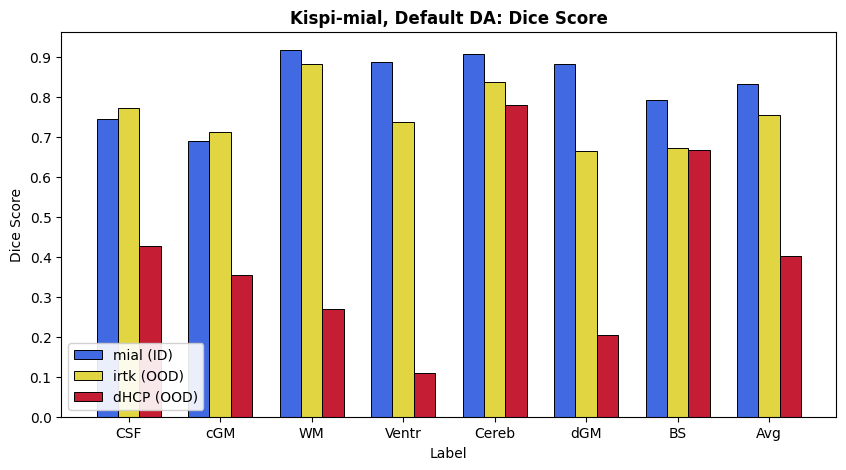
\includegraphics[width=0.8\textwidth]{figures/mial_default_DC.png}\\
    \vspace{10pt}
    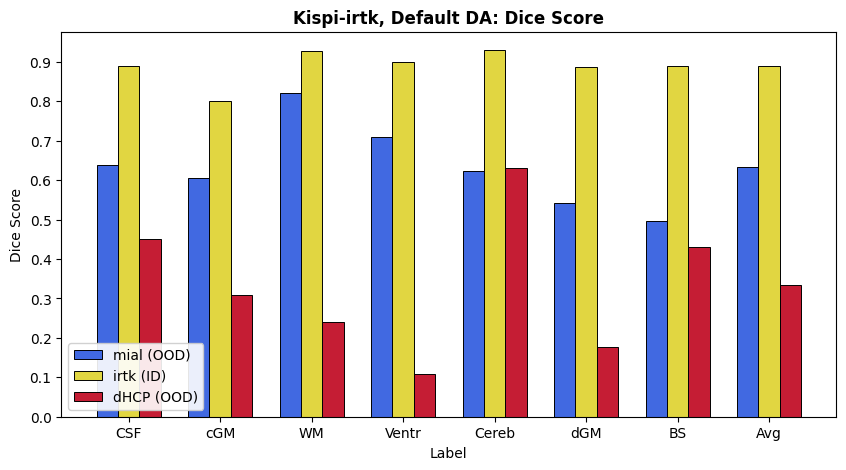
\includegraphics[width=0.8\textwidth]{figures/irtk_default_DC.png}\\
    \vspace{10pt}
    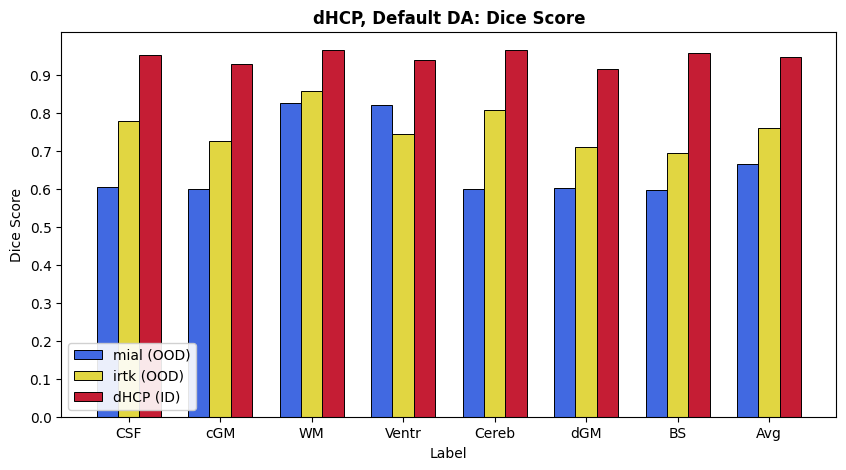
\includegraphics[width=0.8\textwidth]{figures/dHCP_default_DC.png}
    \caption{Dice score across datasets and labels for the nnU-Net default DA (baseline model). From top to bottom: training on Kispi-mial, on Kispi-irtk, and on dHCP.}
    \label{fig:default_DC}
\end{figure}

Although GIN-IPA (see Fig.\,\ref{fig:ginipa_DC}) does not cause an increment in DSC in the models trained on Kispi-mial and dHCP, it produces a significant improvement in the model trained on Kispi-irtk when predicting on dHCP. The raise is mainly located in dGM, ventricles and BS. The average Dice passes from \numrange{0.33}{0.55} (\qty{+66}{\percent}).

\begin{figure}[htbp]
    \centering
    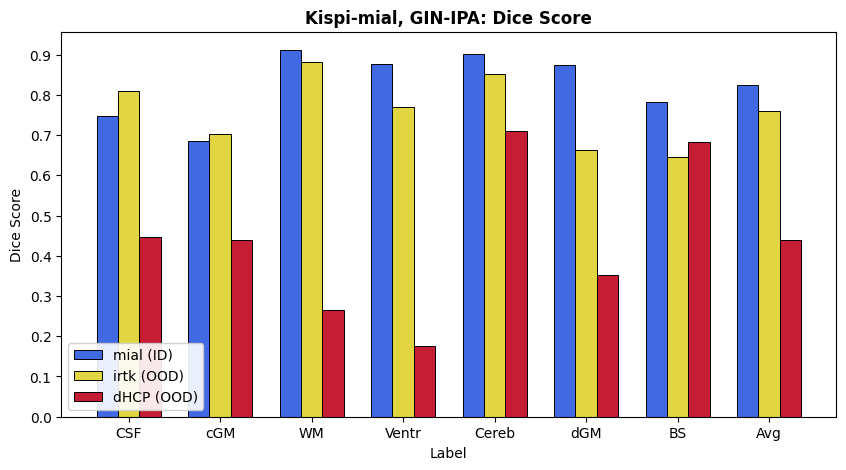
\includegraphics[width=0.8\textwidth]{figures/mial_ginipa_DC.png}\\
    \vspace{10pt}
    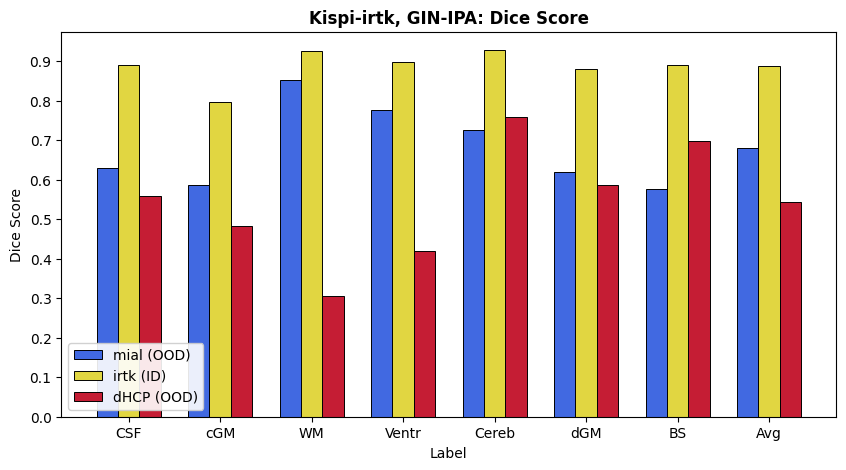
\includegraphics[width=0.8\textwidth]{figures/irtk_ginipa_DC.png}\\
    \vspace{10pt}
    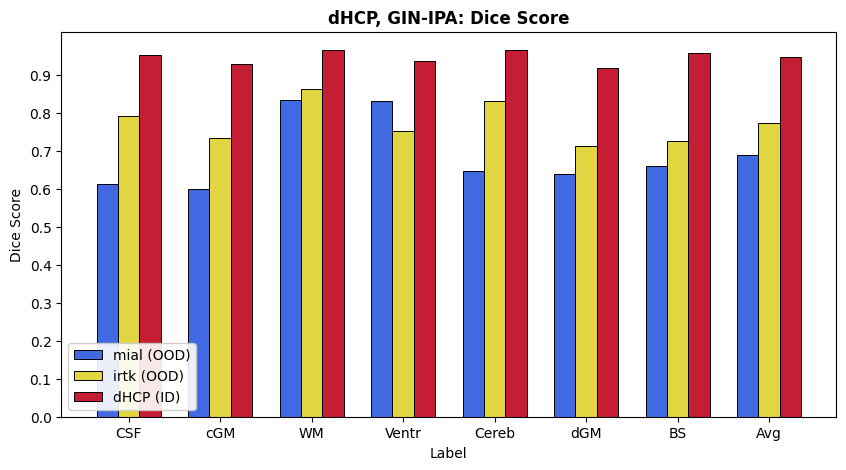
\includegraphics[width=0.8\textwidth]{figures/dHCP_ginipa_DC.png}
    \caption{Dice score across datasets and labels for the GIN-IPA DA model. From top to bottom: training on Kispi-mial, on Kispi-irtk, and on dHCP.}
    \label{fig:ginipa_DC}
\end{figure}

Finally, the model that combines the nnU-Net default DA and GIN-IPA is substantially equivalent to the pure GIN-IPA model (see Fig.\,\ref{fig:both_DC}).

\begin{figure}[htbp]
    \centering
    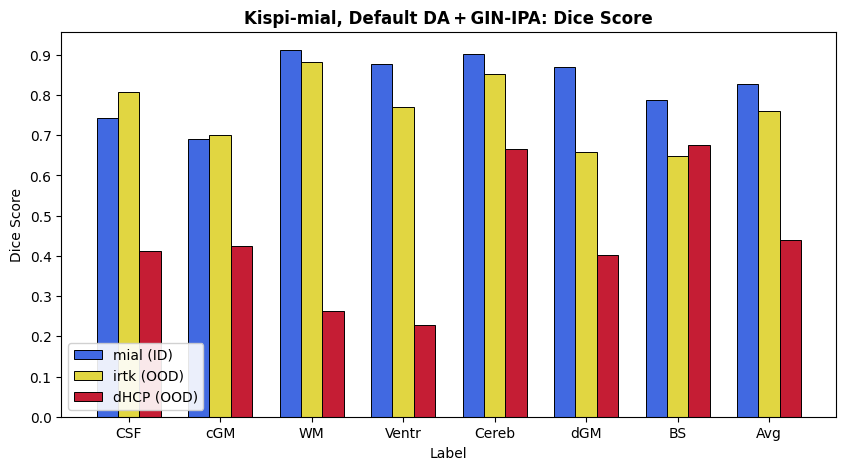
\includegraphics[width=0.8\textwidth]{figures/mial_both_DC.png}\\
    \vspace{10pt}
    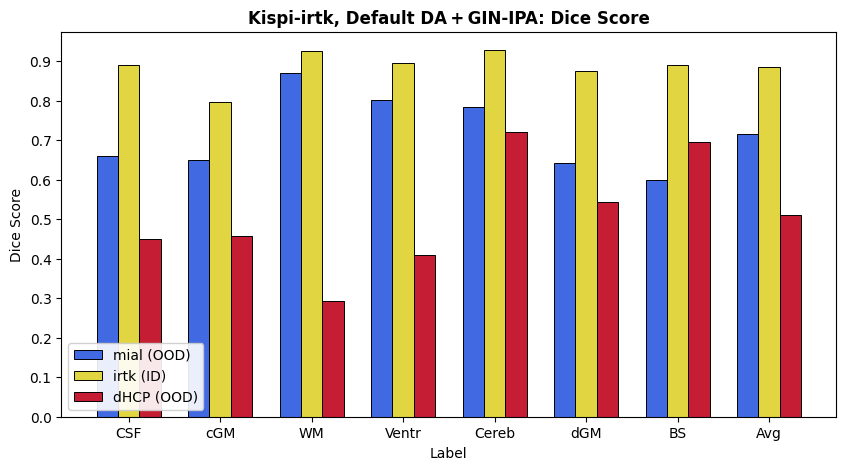
\includegraphics[width=0.8\textwidth]{figures/irtk_both_DC.png}\\
    \vspace{10pt}
    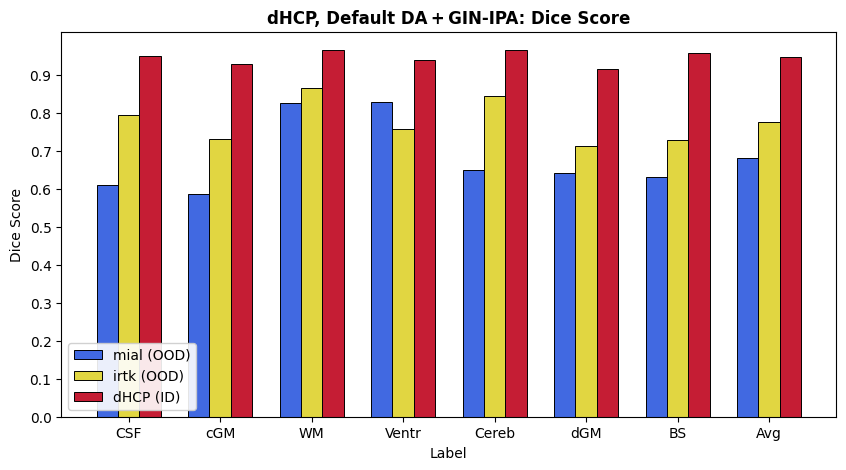
\includegraphics[width=0.8\textwidth]{figures/dHCP_both_DC.png}
    \caption{Dice score across datasets and labels for the combined DA (default\,+\,GIN-IPA) model. From top to bottom: training on Kispi-mial, on Kispi-irtk, and on dHCP.}
    \label{fig:both_DC}
\end{figure}
